%%%%%%%%%%%%%%%%%%%%%%%%%%%%%%%%%%%%%%%%%%%%%%%%%%%%%%%%%%%%%%%%%%%%%%%%%%%%%%%%
%2345678901234567890123456789012345678901234567890123456789012345678901234567890
%        1         2         3         4         5         6         7         8
\documentclass[10pt,conference]{IEEEtran}

%\overrideIEEEmargins                                      % Needed to meet printer requirements.

%In case you encounter the following error:
%Error 1010 The PDF file may be corrupt (unable to open PDF file) OR
%Error 1000 An error occurred while parsing a contents stream. Unable to analyze the PDF file.
%This is a known problem with pdfLaTeX conversion filter. The file cannot be opened with acrobat reader
%Please use one of the alternatives below to circumvent this error by uncommenting one or the other
%\pdfobjcompresslevel=0
%\pdfminorversion=4

% See the \addtolength command later in the file to balance the column lengths
% on the last page of the document

% The following packages can be found on http:\\www.ctan.org
\usepackage{graphicx}
%\usepackage{graphics} % for pdf, bitmapped graphics files
%\usepackage{epsfig} % for postscript graphics files
%\usepackage{mathptmx} % assumes new font selection scheme installed
%\usepackage{times} % assumes new font selection scheme installed
\usepackage{amsmath} % assumes amsmath package installed
\usepackage{amssymb}  % assumes amsmath package installed
\usepackage{bm} % for bold symbols in math mode
\usepackage{cite}

\title{\LARGE \bf
Report: SLIP models for controlling articulated robotic legs
}


\author{Stefan Schneyer and Fabian Kolb}

\begin{document}
\maketitle
\thispagestyle{empty}
\pagestyle{empty}


%%%%%%%%%%%%%%%%%%%%%%%%%%%%%%%%%%%%%%%%%%%%%%%%%%%%%%%%%%%%%%%%%%%%%%%%%%%%%%%%
%\begin{abstract} TODOabstract \end{abstract}

\section{Introduction}
\label{sec:Introduction}


Bio inspired robotics and especially humanoid robots play an increasing role in society and science. Robotic solutions with a structural 
similarity to humans are especially suitable for tasks which are mainly solved by humans. For moving in challenging terrain with higher velocity,
hopping is an interesting approach. For simplicity, hopping is simulated with one leg. SLIP models describe the spring-like leg behavior
of animals and humans in a very simple and abstract way. The SLIP model creates a behavior which is then projected onto the articulated leg. 
In a first stage, a closed loop dynamics is generated based on the SLIP model. In the second stage, the high order robotic leg tracks this closed loop dynamics 
and uses a feedback controller to adapt to perturbations. In our project the robot's state is modelled with a hybrid automaton. 
A continuous state captures the position of the robot in the 3D space, as well as the angle in hip and knee. A discrete state describes whether the robot is 
in the flight to stance phase. A control structure is implemented separately for those two discrete phases. 
For the flight phase, a cascade control consisting of PI and PID controller is used which tracks the landing angle alpha. When touching the ground, the SLIP dynamics 
can be projected onto the center of gravity (CoG) motion of the robotic leg. From there, the joint actuator torques are calculated with the SLIP control law. The articulated robotic leg 
differs from the simplified SLIP model because the mass and inertia of each leg segment influences the robot's motion. This is the reason why the articulated 
leg is influenced by the impact at touchdown. This leads to a velocity change and therefore a loss of kinetic energy. To incorporate that into the SLIP model, an extended 
version SLIPic with impact compensation is used. Different types of solvers are implemented in order to study their effect on the controller stability. 
The project is implemented in Python. The RBDL library is used, which offers efficient rigid body dynamics algorithms. The articulated leg is visualized with Meshup, 
a tool which was developed with RBDL.




\section{SLIP model}
\label{sec:SLIP model}
The SLIP model captures the locomotion behavior of robots with light, compliant legs in an abstract way. The body is reduced to a point mass \( m \). The
leg is represented by a massless spring with stiffness \({k}_0 \) and a rest length \({l}_0 \). For this system the equations of motion are the following:
\begin{equation}
   \begin{bmatrix} m & 0 \\ 0 & m \end{bmatrix}
   \begin{bmatrix} \ddot{x} \\ \ddot{y} \end{bmatrix}
   +
   \begin{bmatrix} 0 \\ mg \end{bmatrix}
   =
   \begin{bmatrix} {F}_{x} \\ {F}_{y} \end{bmatrix},
   \label{eq:equation of motion}
\end{equation}

where \(x\) and \(y\) are the coordinates of the center of mass (COM). \({F}_x \) and \({F}_y \) are the ground reaction forces (GRF). The GRFs are 0 during flight and depend 
on the length of the spring \(l\) during compression and the landing angle \(\alpha\) of the foot.

\begin{equation}
   \begin{bmatrix} {F}_{x}  \\ {F}_{y}  \end{bmatrix}
   =
   {k}_{0} ({l}_{0} -l)
   \begin{bmatrix} -cos(\alpha) \\ sin(\alpha) \end{bmatrix},
\end{equation}

The SLIP model describes running as a series of apex heights \({y}_i \)

\begin{figure}[h]
   \centering
   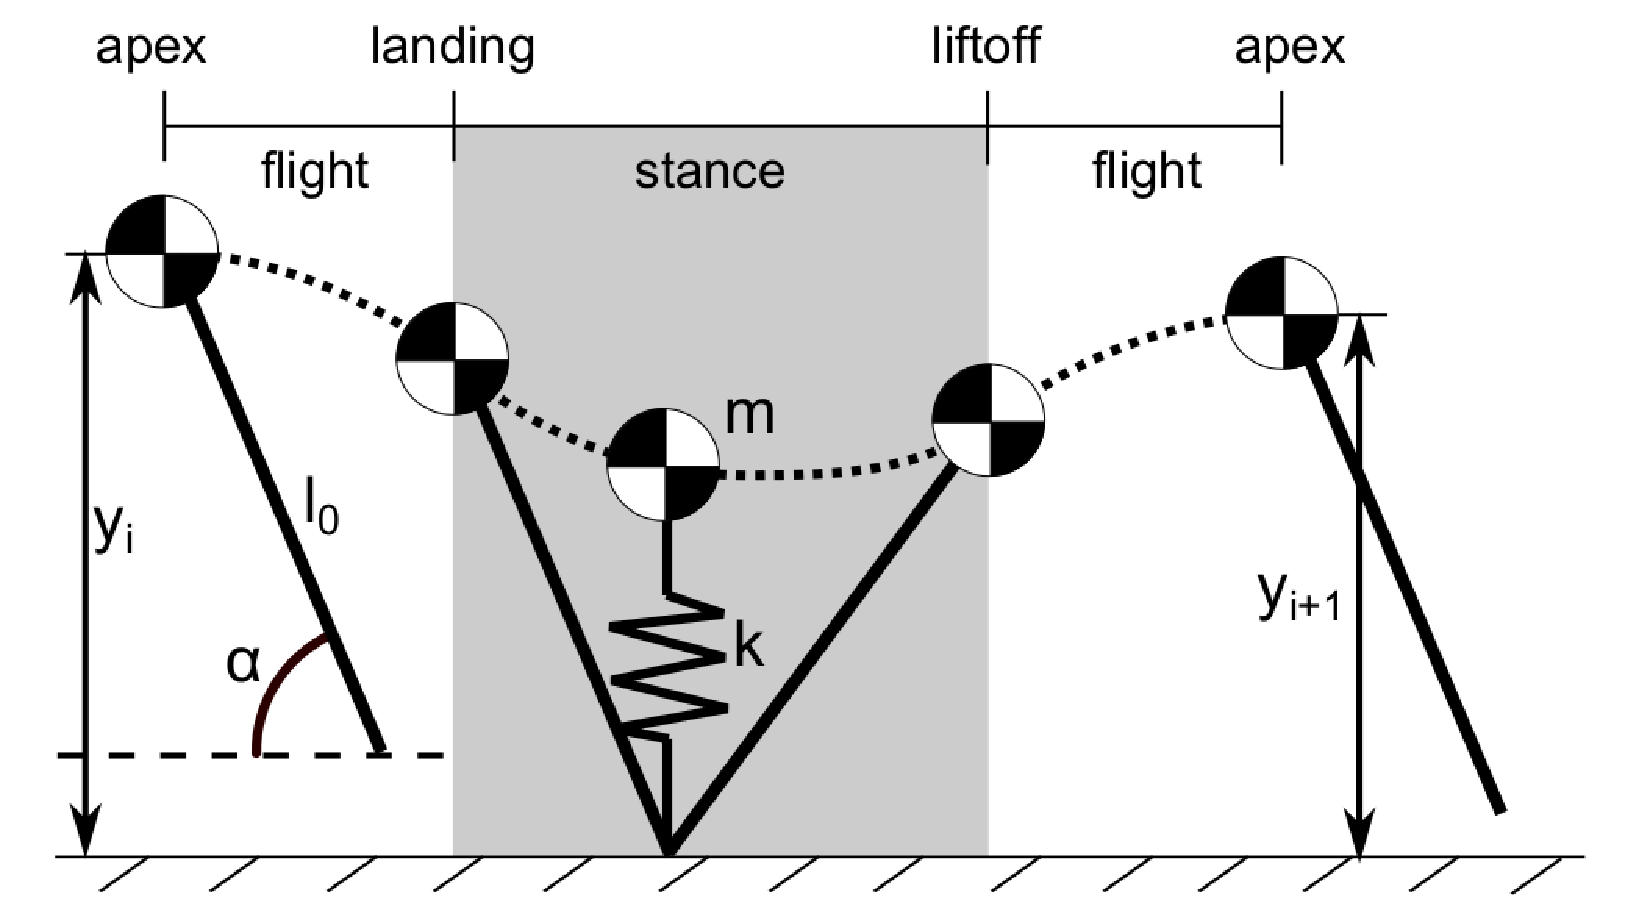
\includegraphics[scale=0.2]{"assets/SMM2.pdf"}
   \caption{Flight and stance phases of SLIP model \cite{Wu2014}}
   \label{fig_SLIP_phase}
\end{figure}


In Fig \ref{fig_SLIP_phase} it becomes clear how the robot trajectory can be separated in flight and stance phases. The gait behavior is characterized by the forward speed and the apex height.
The SLIP model is a conservative system without any friction or other mechanism to dissipate the dynamics, and thus, the phase space does not shrink over time. 
Therefore, the apex height and forwards speed are coupled through the system energy and the trajectory is fully characterized by the apex height. 
The transition between two consecutive apex heights is defined by the landing angle \(\alpha\):
\begin{equation}
   {f}_{yi+1}={f}_{yi}|(\alpha),
\end{equation}
The landing angle is used to achieve deadbeat stability of the system \cite{Wu2014} \cite{Hutter2010}.




\section{Control}
\label{sec:Control}
Different control designs were used for the flight and stance phase. 

\subsection{Stance control}
The mechanics of a robotic leg under support conditions is the following:
\begin{equation}
   M(q)\ddot{q}+b+g+{J}_{s}^{T}F_{s}=S^{T}{\tau},
\end{equation}

with the mass matrix M , the coriolis and centrifugal force vector b , the gravitational force g , the ground contact force
$F_s$, the corresponding support Jacobian \({J}_{s}\), the actuation torques \(\tau = [{\tau}_{Hip}, {\tau}_{Knee}]^{T}\) and the actuator selection matrix S
limiting the actuation to hip and knee joints. The generalized coordinates  \(q = [x_{MainBody}, y_{MainBody}, {\phi}_{Hip}, {\phi}_{Knee}]^{T}\)
describe the current robot state. Since we assume no slip between foot and ground during contact. The following conditions apply: 
\begin{equation}
   \dot{x}_{s} = J_{s} \dot{q} = 0,
\end{equation}
\begin{equation}
   \ddot{x}_{s} = J_{s} \ddot{q} + \dot{J}_{s} \dot{q}=0,
\end{equation}

This reduces the mechanics of a robotic leg to a support consistent description:
\begin{equation}
   M \ddot{q} + {N}_{s}^{T}(b + g) + {J}_{s}^{T} {\Lambda}_{s} {\dot{J}}_{s} \dot{q} = {(S {N}_{s})}^{T} \tau,
\end{equation}

with the support space inertia Matrix \({\Lambda}_{s} = {({J}_{s} {M}^{-1} {J}_{s}^{T})}^{-1}\) and the support nullspace 
\({N}{s}=[I-{M}^{-1} {J}_{s}^{T} {\Lambda}_{s} {J}_{s}]\). The real articulated leg has inertia and mass in each leg segment. Therefore it is affected 
by the impact when the foot hits the ground. The change of the generalized velocity is described by the nullspace \({\dot{q}}^{+}={N}_{s} {\dot{q}}^{-}\)
The stance dynamics can now be projected onto the center of gravity (CoG) of the articulated leg. This allows to compute the operational space force F:
\begin{equation}
   {\Lambda}^{*} {\ddot{r}}_{CoG} + {\mu}^{*} + {p}^{*} = F, 
   \label{eq:operational space force F}
\end{equation}
The operational space force F do relate to the robot actuation like the following:
\begin{equation}
   \tau = {J}^{*T}F,
   \label{eq:tau from operational space force F}
\end{equation}

The different terms which are used in \ref{eq:operational space force F} and \ref{eq:tau from operational space force F} are presented in the following:\\* 
i) task interia: 
\begin{equation}
   {\Lambda}^{*} = {(J {M}^{-1} S {N}_{s} {J}^{*})}^{-1}, 
\end{equation}
ii) projected coriolis and centrifugal terms
\begin{equation}
\begin{aligned}
   {\mu}^{*} = & \ {\Lambda}^{*} {J}_{CoG} {M}^{-1} {N}_{s}^{T} b - {\Lambda}^{*} {\dot{J}}_{CoG} \dot{q} \\
   & \ + {\Lambda}^{*} {J}_{CoG} {M}^{-1} {J}_{s}^{T} {\Lambda}_{s} {\dot{J}}_{s} \dot{q},\
\end{aligned}
\end{equation}
iii) projected gravitational term
\begin{equation}
   {p}^{*} = {\Lambda}^{*} {J}_{CoG} {M}^{-1} {N}_{s}^{T} g,
\end{equation}
iv) support reduced Jacobian
\begin{equation}
   {J}^{*} = {J}_{CoG} {M}^{-1} {(S {N}_{s})}^{T} {(S {N}_{s} {M}^{-1} {(S {N}_{s})}^{T})}^{-1}
\end{equation}

After projecting the stance dynamics of the robotic leg onto its CoG, the SLIP dynamics can be imposed on the CoG motion of the articulated leg. 
Then the equations of motion of the SLIP model 
in \ref{eq:equation of motion} can be solved for the \(\ddot{x}, \ddot{y}\) which are then be inserted for \({\ddot{r}}_{CoG}\) in \ref{eq:operational space force F}. This 
enables the SLIP control law:
\begin{equation}
   \tau = {J}^{*T} ({\Lambda}^{*} \frac{1}{m} ({F}_{leg} + mg) + {\mu}^{*} + {p}^{*})
\end{equation}
If we assume to have a perfect model of the articulated leg and the CoG motion of the SLIP model is feasible, using the SLIP control law the CoG of the articulated leg will 
follow the SLIP trajectory accuratly. This paragraph follows Hutters work in \cite{Hutter2010}


\subsection{Flight control}
A cascade control is used in the flight phase to track the landing angle \(\alpha\). The cascade control consists of two PI and one PID controller and is shown in Fig \ref{fig:cascade}. 
The position controller uses the difference of the goal and current position of the CoG to calculate the desired velocity of the CoG. The velocity controller uses 
the difference of the goal and current velocity of the CoG to calculate the desired angle of attack in the SLIP model. From this angle, the goal foot position can be 
calculated. This foot position is compared with the current foot position of the articulated leg and a desired acceleration of the foot is set. From there the torques 
required to generate this acceleration is estimated. The relation between joint accelerations and end-effector accelerations is given by the 
Jacobians. To transform the accelerations in the joints to robot actuation the mass matrix and Newton's first law is used.

\begin{figure}[h]
   \centering
   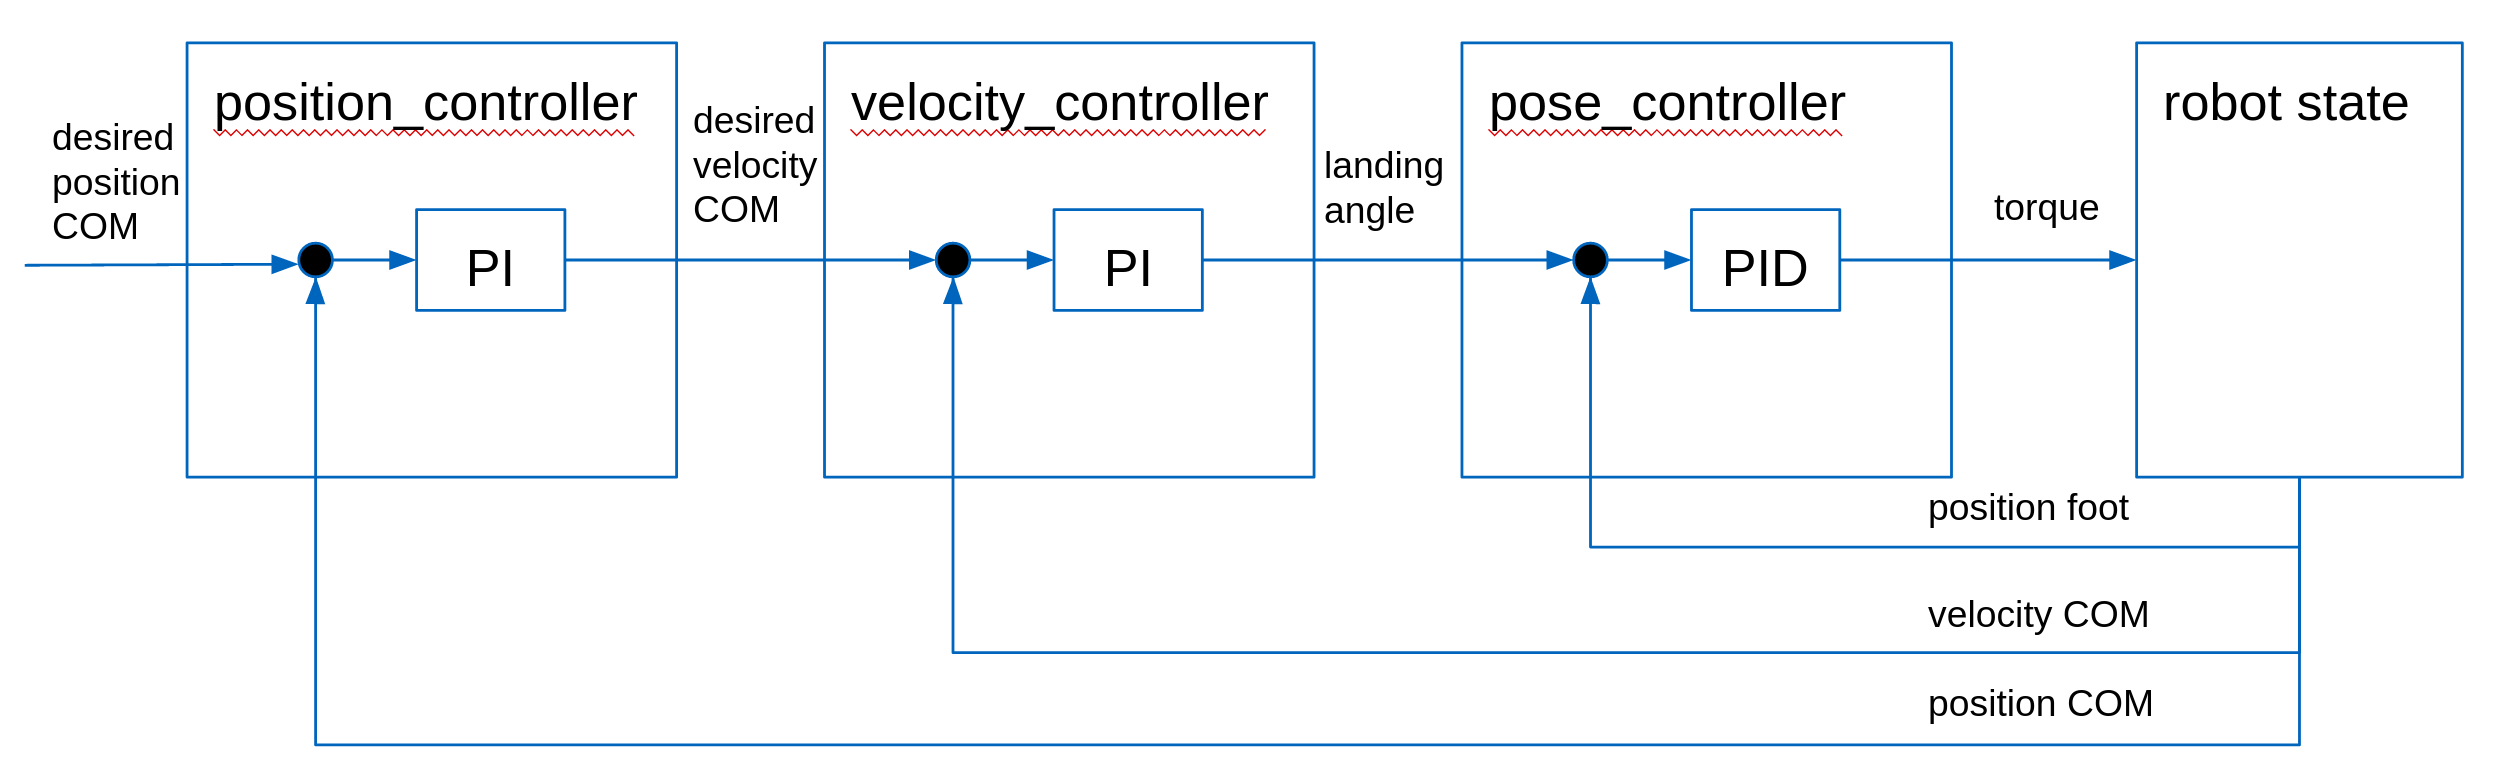
\includegraphics[scale=0.11]{"assets/cascade.png"}
   \caption{Flight control}
   \label{fig:cascade}
\end{figure}

\section{SLIPic}
\label{sec:SLIPic}
For the SLIP model, the leg is modeled with a massless spring. In reality, the articulated leg does have mass and inertia in each segment of the leg. 
The impact at touchdown influences the velocity of the articulated leg. Therefore the generalized velocity changes through the impact. 
Like mentioned earlier, this velocity change is described through the support nullspace. This velocity change leads to a loss of kinetic energy:
\begin{equation}
\begin{aligned}
   \Delta E = & \ 0.5 {m}_{CoG} ({|{\dot{r}}_{CoG}^{-}|}^{2} - {|{\dot{r}}_{CoG}^{+}|}^{2}) \\
   & \ =0.5 {m}_{CoG} {\dot{q}}^{-T} ({J}_{CoG}^{T} {J}_{CoG} - \\
   & \ {N}_{s}^{T} {J}_{CoG}^{T} {J}_{CoG} {N}_{s}) {\dot{q}}^{-},
\end{aligned}
\end{equation}

The SLIP model does not account for that energy loss. If the normal SLIP model is used for the SLIP 
control law in the stance phase this energy loss is not compensated. The potential energy is reduced by the loss of kinetic energy in every jump. This leades to a reduced apex height 
in every foot strike. To prevent that an extended SLIP model is used which considers the loss of kinetic energy through the impact. This model is called SLIP with impact compensation 
(SLIPic). In this model the spring of the SLIP model is pre-compressed at the landing such that the loss of kinetic energy in the articulated leg equals the energy stored in the spring: 

\begin{equation}
   \Delta E = 0.5 k {\Delta l}^{2},
\end{equation}

The spring forces in the SLIP model and therefore also the ground reaction forces (GRF) in the articulated leg are increased such that the energy loss is compensated and the apex height is 
held constant. Fig \ref{fig:SLIPic} visualizes how the virtual spring energy compensates the loss of kinetic energy.

\begin{figure}[h]
   \centering
   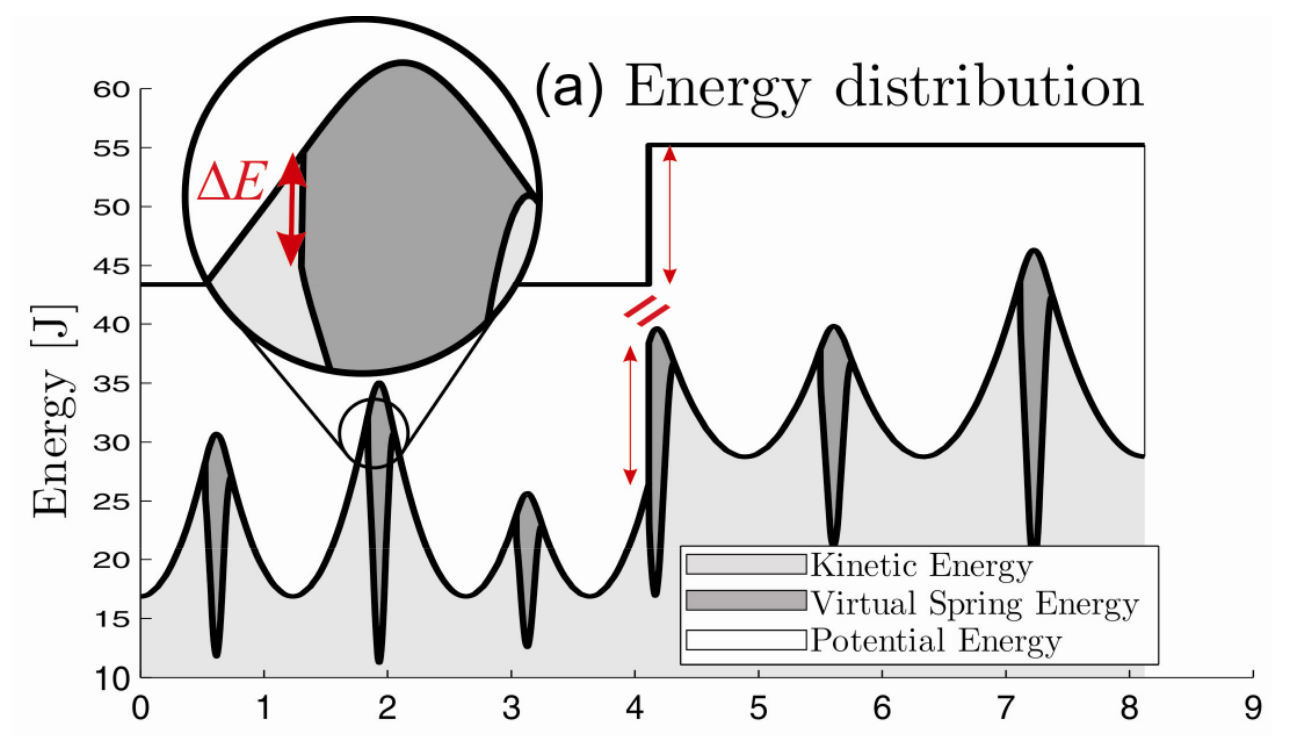
\includegraphics[scale=0.15]{"assets/SLIPic.png"}
   \caption{Impact compensation in SLIPic \cite{Hutter2010}}
   \label{fig:SLIPic}
\end{figure}

\section{Structure}
\label{sec:Structure}
\subsection{Hybrid Automaton}

As mentioned before, the state of the robot leg is described by four continuous values, where two degrees of freedom are used for the position and two more for the leg joints. However, the overall state of the phases, flight and stance, is represented as a discrete state. Since we model both discrete and continuous states, we use a hybrid automaton to simulate the motion of the robot leg. A hybrid automaton is an extended form of a finite state automaton and is formally defined as a tuple:

$$ HA = (Z, X, U, Y, U_c, Y_c, T, inv, g, h, f, z_0, x_0) $$ 

The variable $Z$ is the set of discrete states, which in our case corresponds to the two states for the flight and stance phases. The continuous state space $X$, on the other hand, defines the state of the robot leg given by the four degrees of freedom, the floating base and the joints. $z_0$ and $x_0$ are the initial values for these states. $U$, $Y$, $U_c$ and $Y_c$ are the sets of input and output symbols that we do not use for the simulation. The set of transitions is denoted by $T$ and in our case is the discrete change of state from flight to stance phase, the landing event, and  from stance to flight, the jumping event. The invariant function $inv$, the guard function $g$, the jump function $h$ and the flow function $f$ are used to model the behavior of the continuous state. The invariant is a function that assigns the corresponding continuous subspace to each discrete state.  The guard functions represent the transitions in the continuous state space, such that the guard function assigns subspaces from $X$ to the transitions and separates the subspaces of the invariant functions. The flow function is the differential equation describing the dynamics of the overall system for each discrete state. The jump function is applied to the continuous state when a transition of discrete states occurs. Thus, a jump function exits for each transition.

\begin{figure}[h]
	\centering
	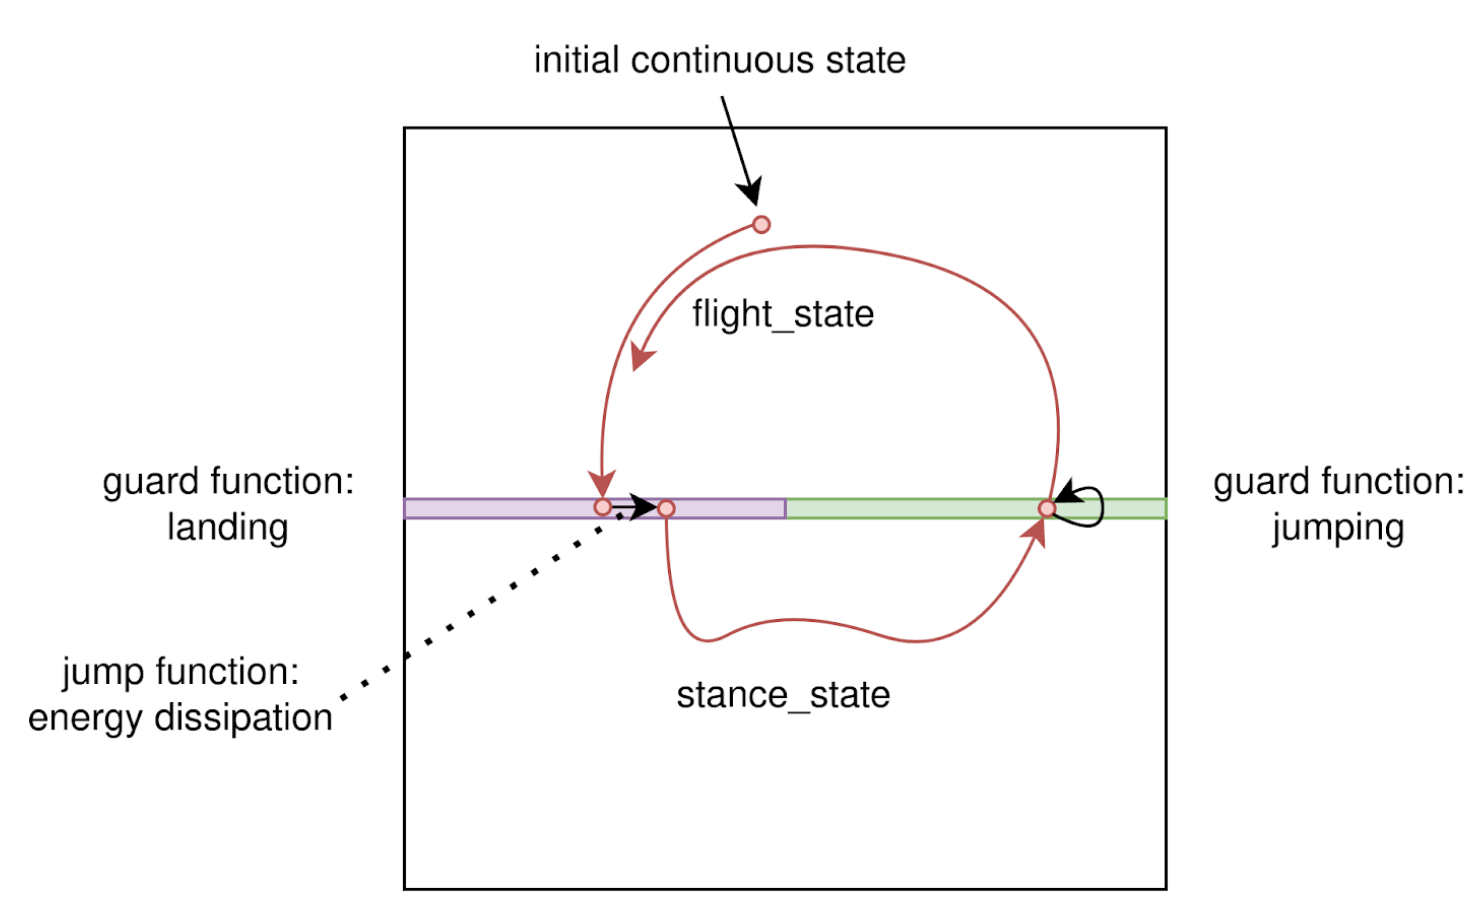
\includegraphics[scale=0.17]{"assets/hybrid_automaton.png"}
	\caption{Hybrid automaton}
	\label{fig:hybrid_automaton}
\end{figure}

The Fig \ref{fig:hybrid_automaton} shows a schematic visualization of the hybrid automaton. To illustrate the concept of a hybrid automaton, the continuous state space is shown qualitatively in a low dimensional representation. The continuous state space for the robot leg actually consists of four or, with derivatives, eight dimensions, which are reduced to two dimensions here. The simulation starts with the initial states. In this case, these are the discrete flight state and the continuous state, shown as a red point. The invariant function defines the rectangular subspaces for flight and stance state. We can now solve the differential equation (flow function) for small time steps and the continuous state is simulated over time, shown as a red line. At the boundary of the flight region, the state enters the landing guard function, which induces the discrete state transition. This executes the corresponding jump function which maps the continuous end state of the flight phase to the state for the stance phase. On landing, the foot hits the ground and loses kinetic energy due to an inelastic impulse. This energy dissipation is modeled using this jump function. Analogously, there is a guard function for the jumping event, green region. However, no energy is lost in this transition.


\subsection{Implementation}
Using the theoretical structure of a hybrid automaton, we model our simulation software for the robot leg. We wrote the Python program in a object-oriented programming manner. The main classes can be see in Fig \ref{fig:class_diagram}. The central class is the hybrid automaton itself, which stores the current discrete and continuous state of the system and uses a solver to simulate the dynamics by integrating the differential equation in small steps. Since we used different solver implementation, we decoupled the different approaches through an interface so that even more implementations can be easily added and used in the project environment. For each discrete state, there is a separate class that implements the flow function, the dynamics of the system, which consists of a controller part and the forward dynamics of the robot leg. Since only the controller iteration of the flow function differs between the states, we use an abstract class that implements both the flow and the forward dynamics of the system. Only the controller is then designed to be state-specific. In the flight phase, we use multiple PID controllers, so it was helpful to add an separate class for this functionality.

\begin{figure}[h]
   \centering
   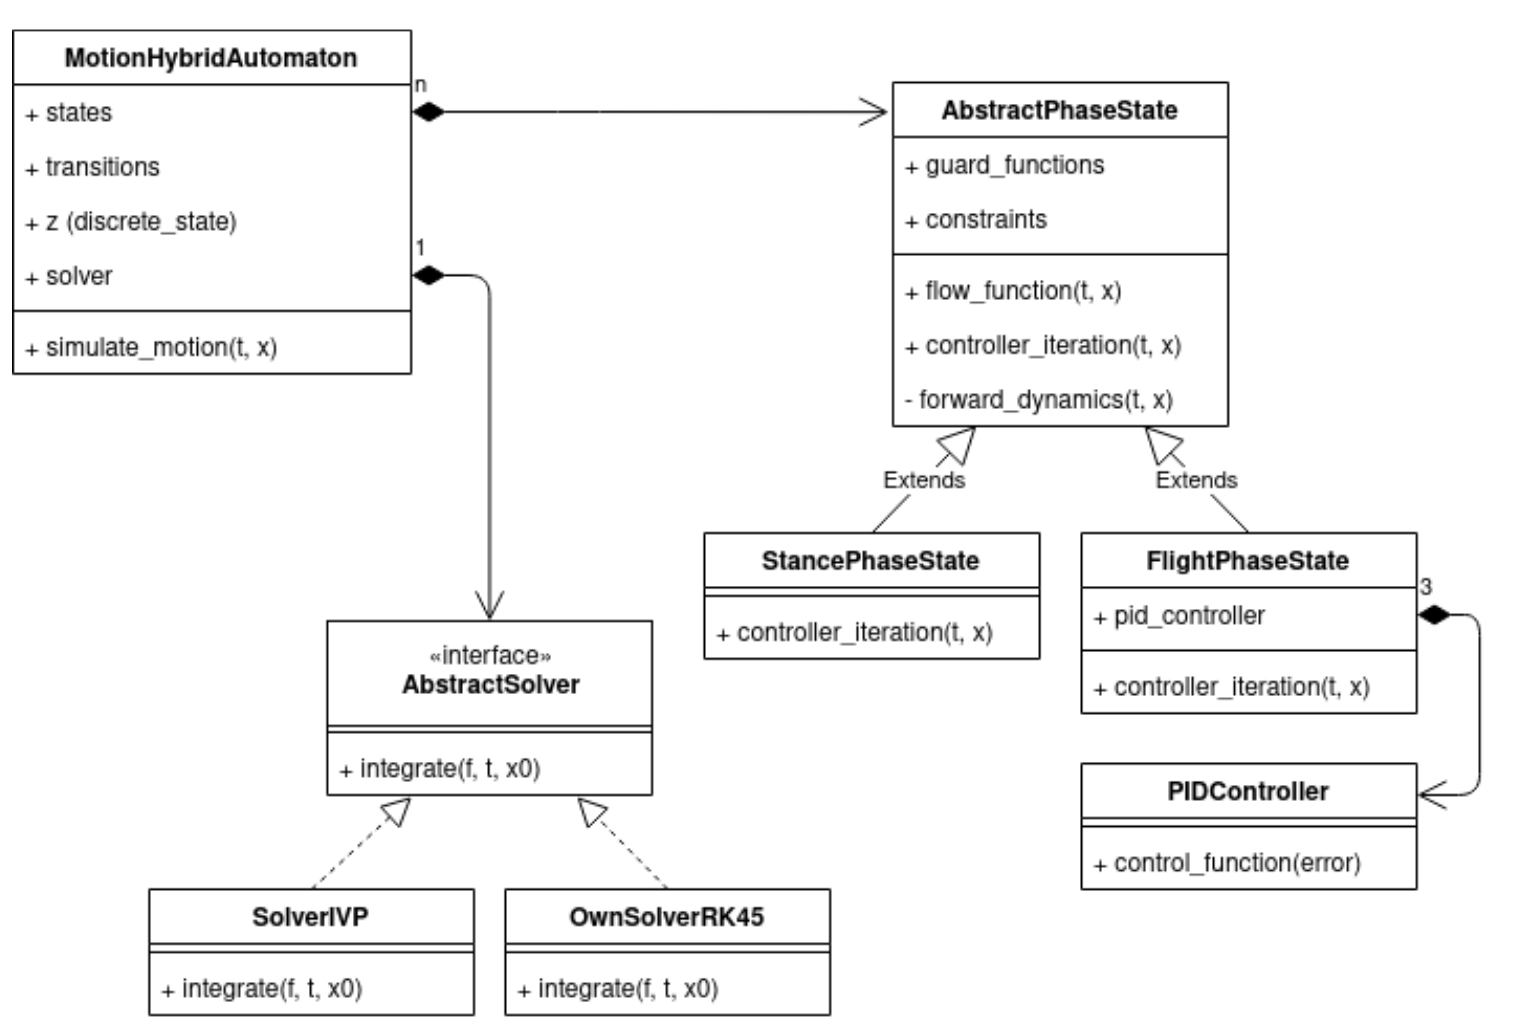
\includegraphics[scale=0.17]{"assets/class_structure.png"}
   \caption{Class diagram}
   \label{fig:class_diagram}
\end{figure}

\section{Solver}
\label{sec:Solver}
To calculate the robots state we iteratively do a control, forward dynamics and integration step. In the control step we calculate the required robot actuation from 
the current robot state. For this we use our stance and flight controller described in Section \ref{sec:Control}. In the forward dynamics the robot state derivative 
is calculated from the current robot state and the robot actuation. Integrating this robot state derivative returns the robot state for the next time step. The step size 
of the solver loop determines the accuracy of the solution for the robot state. The step size is determined by the steps the integrator takes.


\begin{figure}[h]
   \centering
   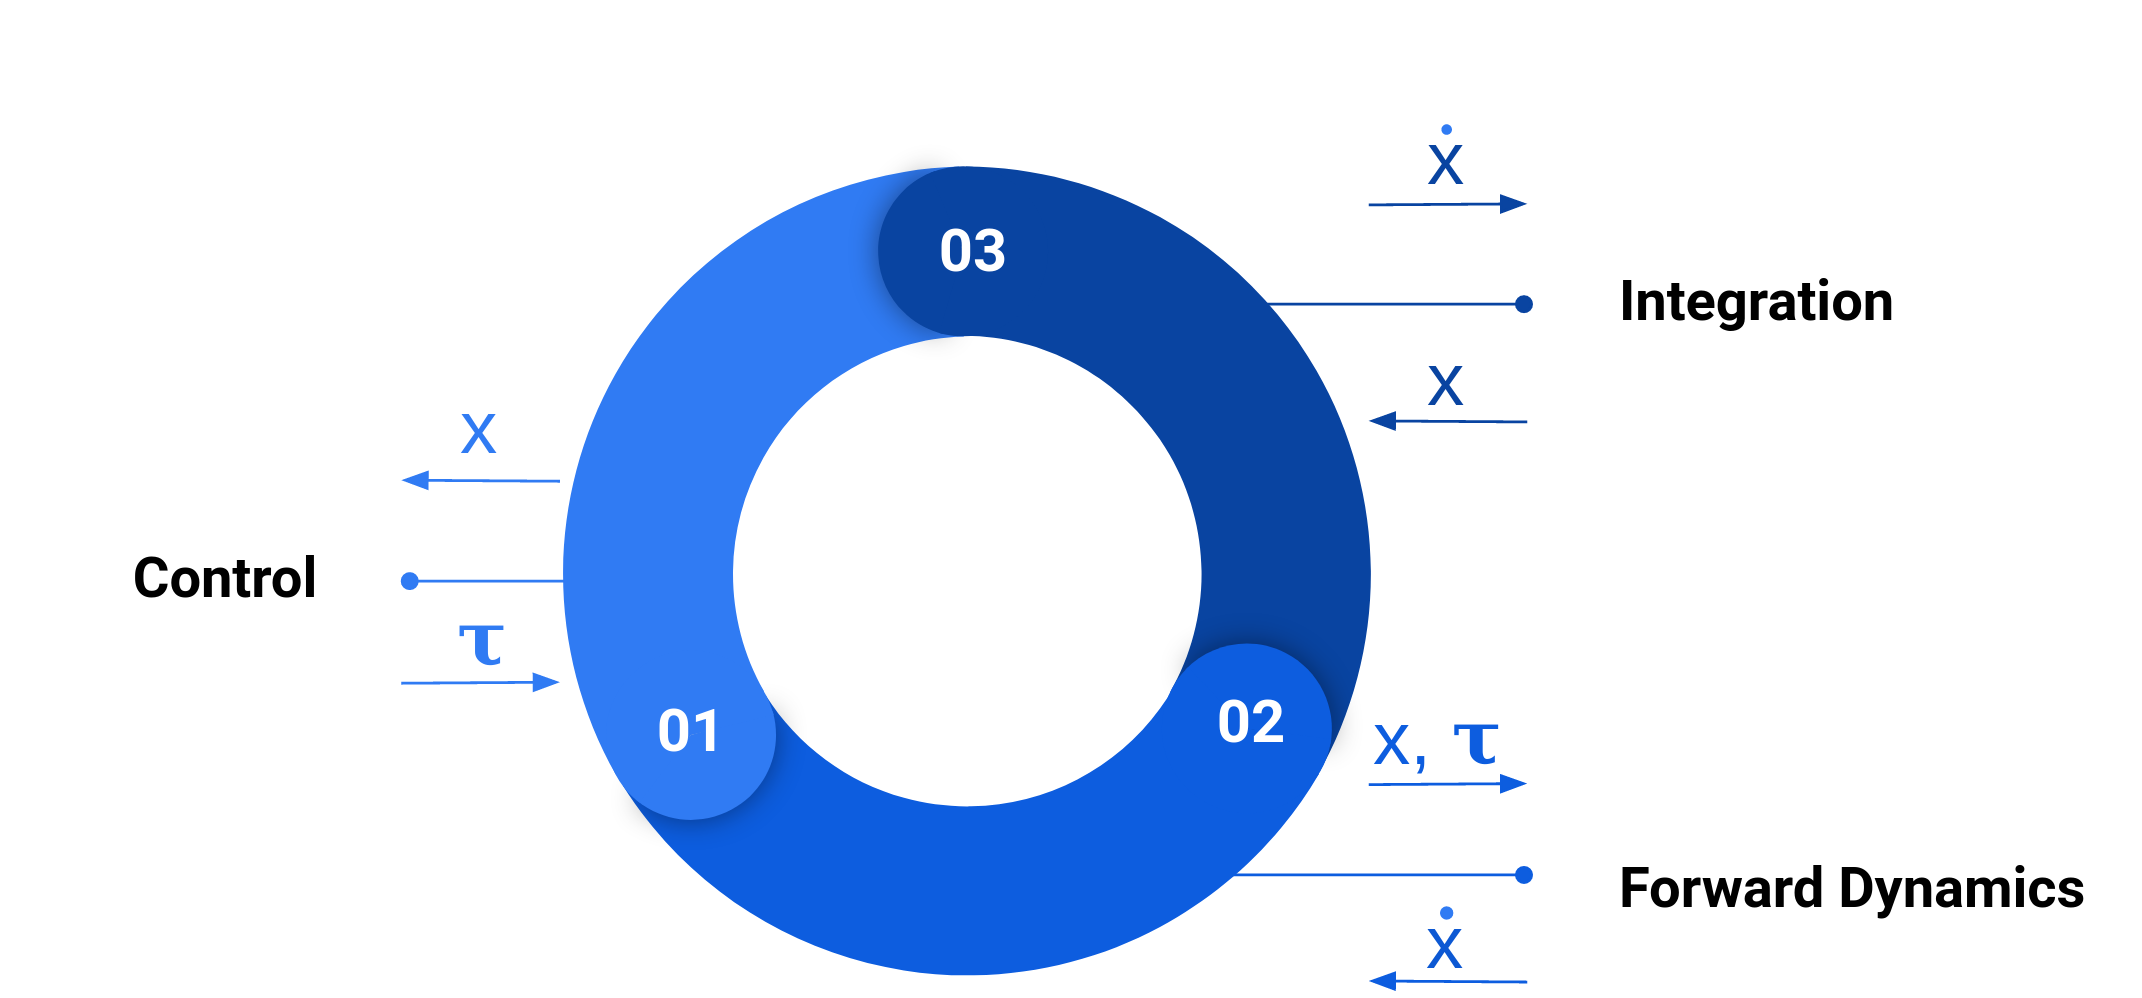
\includegraphics[scale=0.12]{"assets/solver_iteration.png"}
   \caption{Solver iteration}
   \label{fig:solver_iteration}
\end{figure}

In each iteration, a state transition from stance to flight or flight to stance phase is checked. The jump function uses the solved robot state from this solver iteration 
to calculate the discrete state transition. 
In a first attempt, the ivp solver by SciPy is applied. This solver uses the Runge-Kutta method of order 5(4) to numerically integrate a system of ordinary differential 
equations given an initial value. The robot state derivative is integrated until the end of the integration interval is reached, or an event function is 
fulfilled.  The guard functions which mark the transition between the discrete states are used as event functions. Using root-finding the ivp solver will find an 
accurate robot state at time t when the event function is zero. This has the advantage that the robot state is known exactly at the state transition and can be used 
in the jump functions. The ivp solver uses variable step size for each integration step. This variable step size causes unstable behavior in the system. The PID 
controller in the flight control numerically differentiates the foot position error. A numerical differentiation with a variable time interval causes stability 
problems and makes tuning the PID controller hard. Fig \ref{fig:ivp solver} shows that after 4 jumps the system becomes unstable.

\begin{figure}[h]
   \centering
   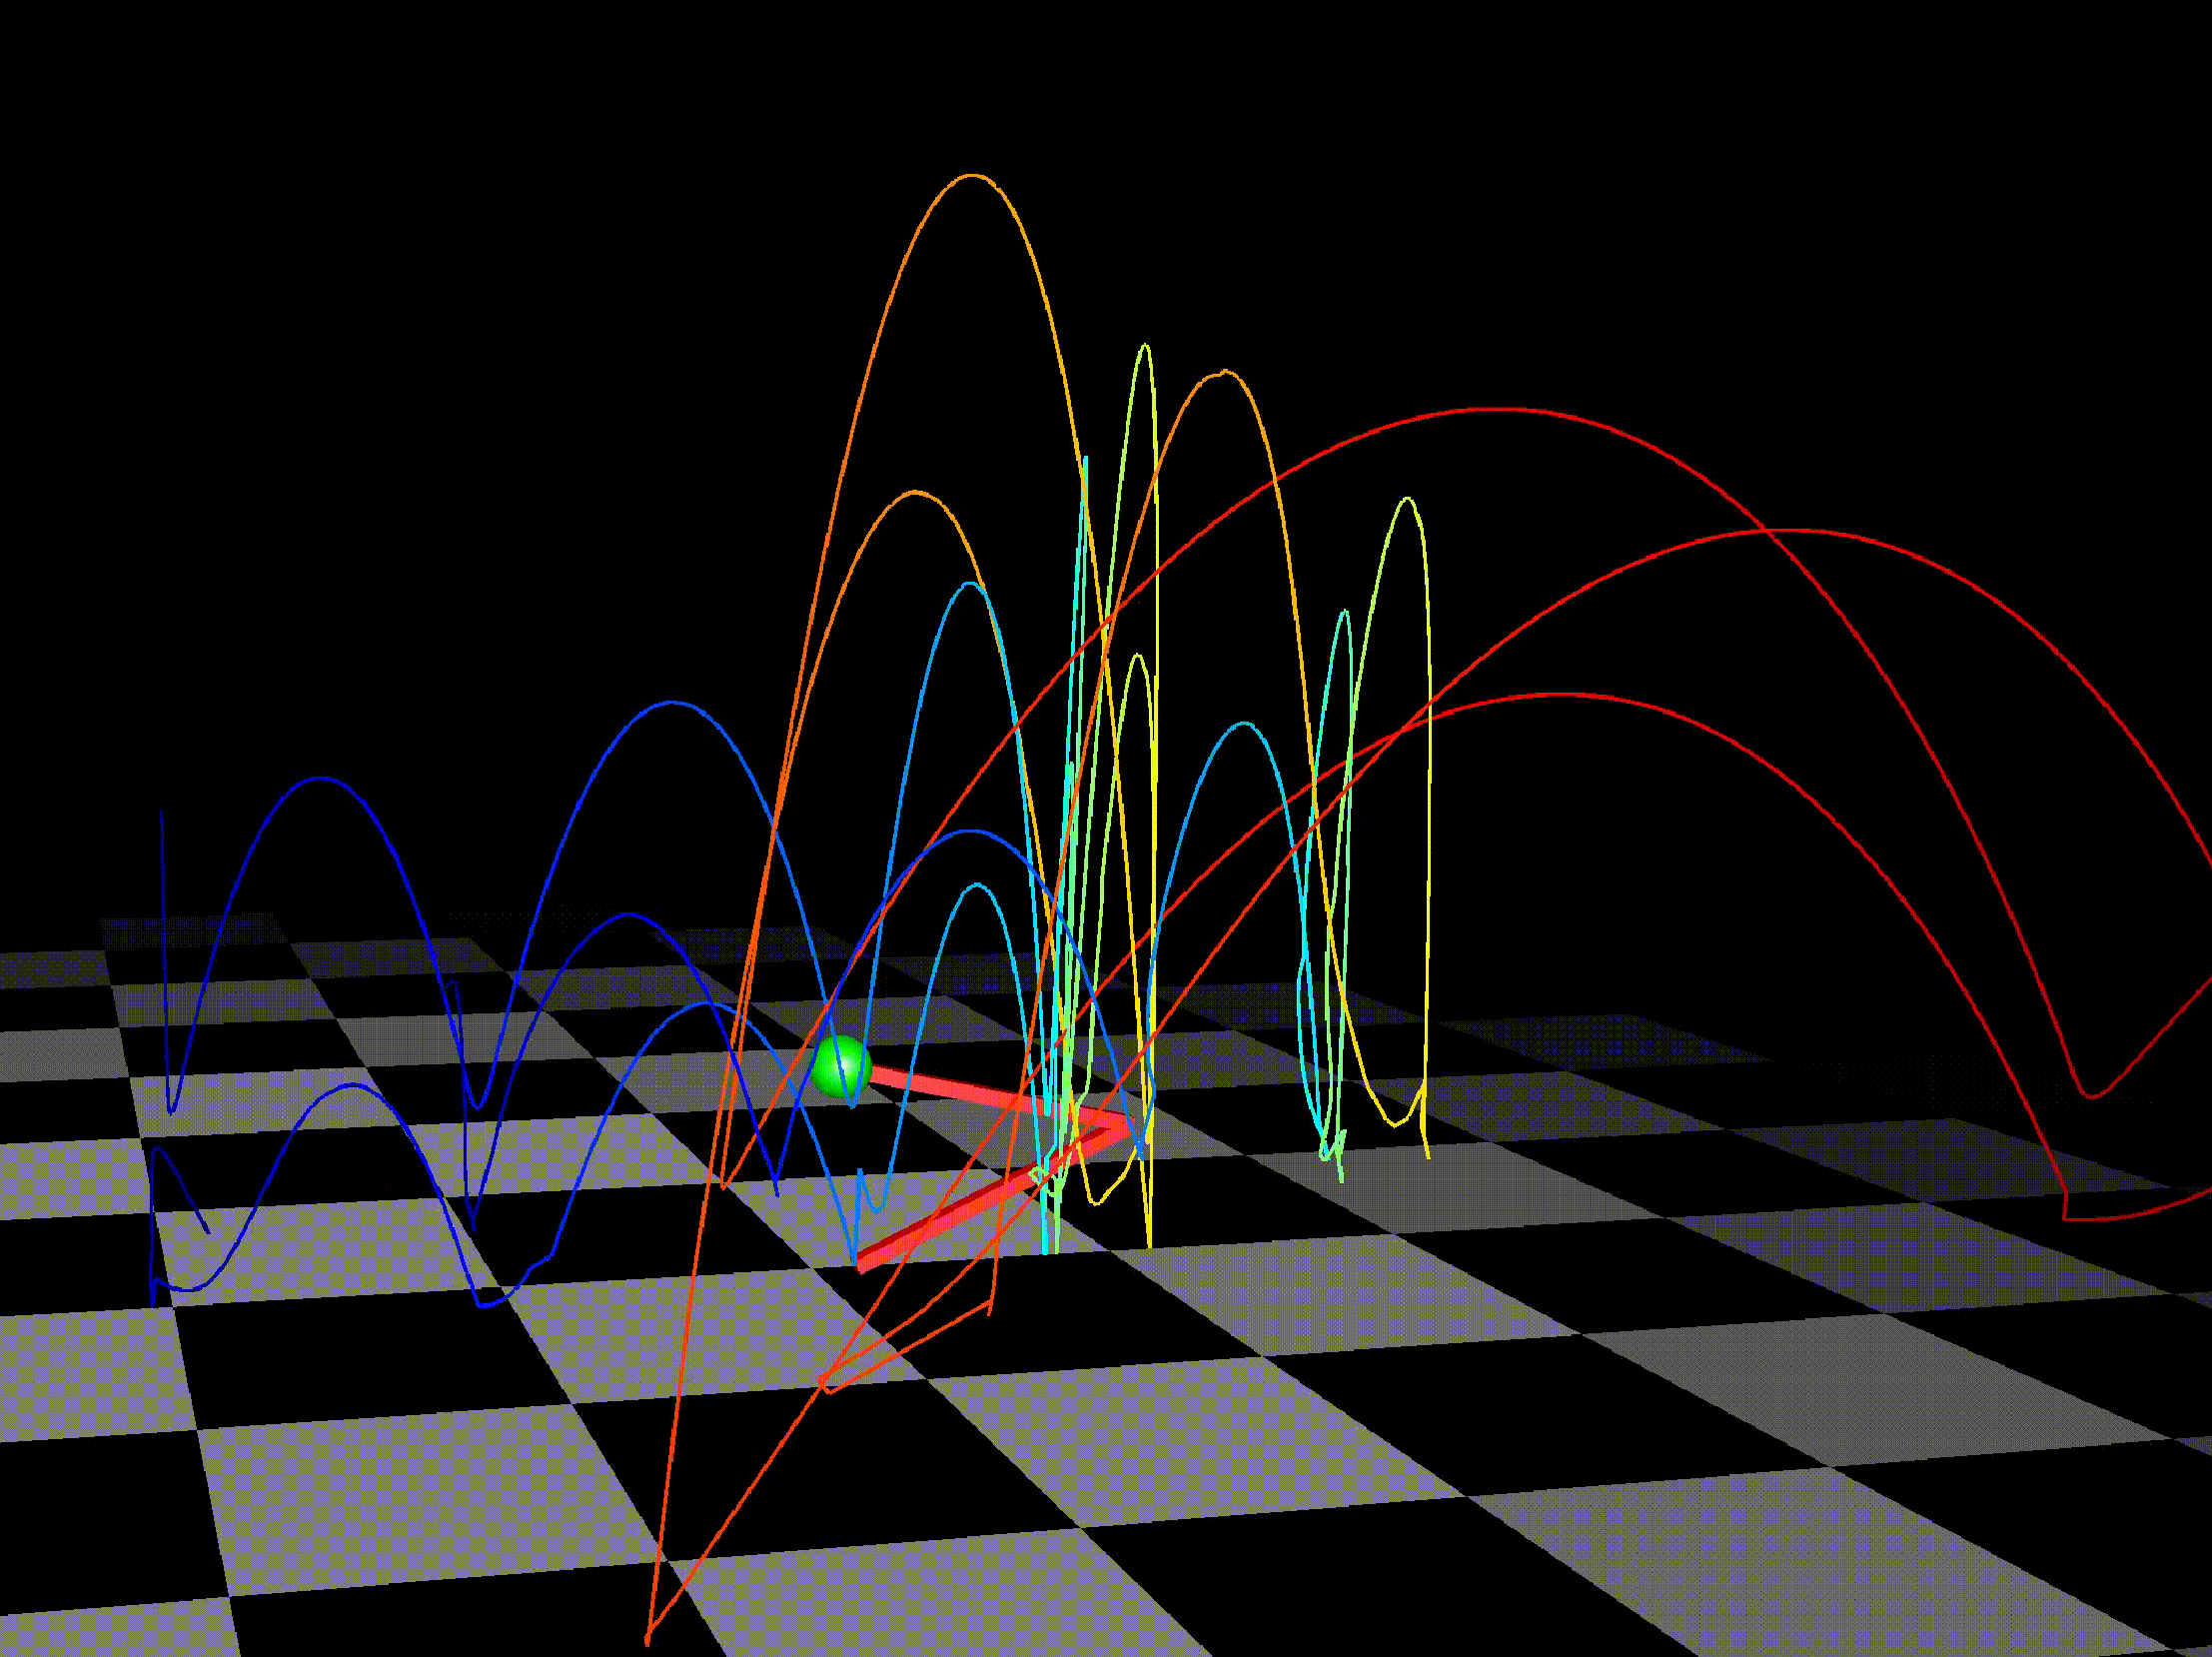
\includegraphics[scale=0.11]{"assets/solver_ivp.png"}
   \caption{Ivp solver}
   \label{fig:ivp solver}
\end{figure}

In a second attempt, the Runge-Kutta method of order 5(4) with a fixed step size is implemented and evaluated. This has the disadvantage that no root-finding is used. 
After each integration step, the guard functions are checked to make sure whether a discrete state transition did occur. Compared to the ivp solver the robot state at 
the transition event is not as accurate since no root-finding is used. Choosing a small enough step size makes this problem insignificant. The fixed step size helps 
a lot to make the flight controller more stable. Fig \ref{fig:RK45 solver} shows the good results with this method.

\begin{figure}[h]
   \centering
   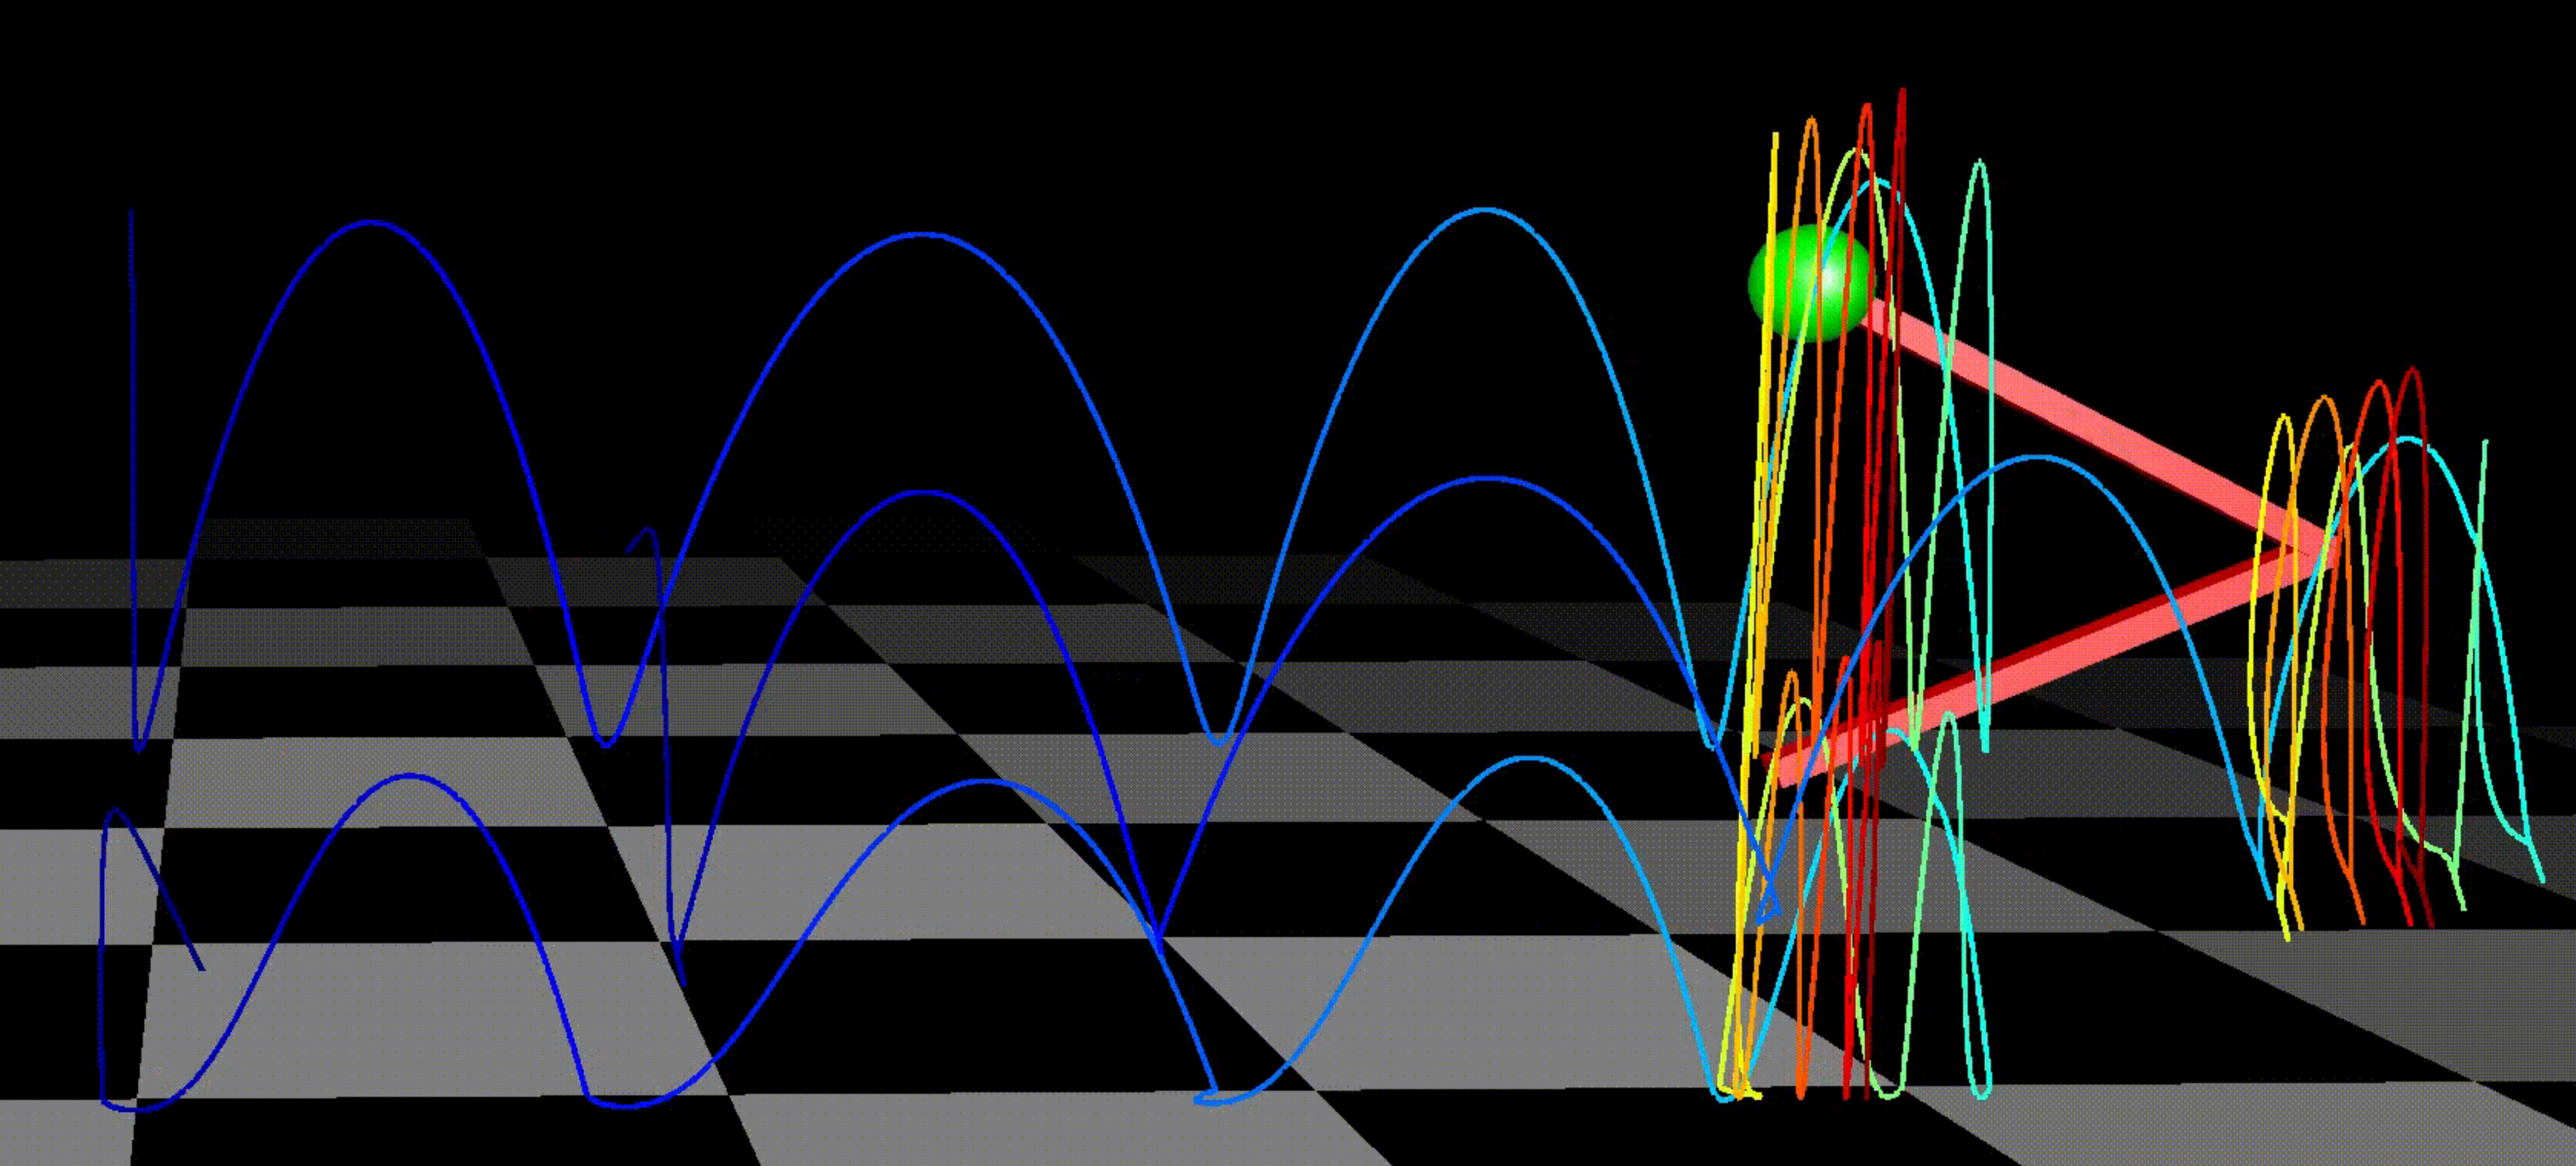
\includegraphics[scale=0.074]{"assets/solver_rk45.png"}
   \caption{RK45 solver}
   \label{fig:RK45 solver}
\end{figure}

\section{Summary}
The very low level SLIP model was implemented sucessfully to control the high level robotic leg. To keep a constant apex 
height through all foot strikes, the extended SLIP model SLIPic was used in this project. The flight control caused some problems in the beginning but was solved by using a 
solver with fixed step size. The project was implemented in a very modular, generic and extensible way, such that future projects can use this implementation to 
develop a more sophisticated control structure or to extend the articulated leg to a more complex one.

\section{Conclusion}
Overall, the control of the articulated leg works good. It was a challenge to detect the robot state exactly at the discrete state transition with the RK45 solver.
In the future, this issue could be improved by either using a solver which finds the exact state transition event or using a control structure which does not 
separate between flight and stance phase. A controller which controls the articulated leg in the stance and the flight phase would be more elegant. 
Extending the articulated leg to an even more realistic one or including a second leg or an upper body would also be a great future project.


\addtolength{\textheight}{-12cm}   % This command serves to balance the column lengths
                                  % on the last page of the document manually. It shortens
                                  % the textheight of the last page by a suitable amount.
                                  % This command does not take effect until the next page
                                  % so it should come on the page before the last. Make
                                  % sure that you do not shorten the textheight too much.

\nocite{*}
\bibliographystyle{IEEEtran}
\bibliography{IEEEabrv, report}

\end{document}
